\chapter{Optimisation} \label{cha:Optimisation}
\section{Introduction} \label{sec:Optimisation-Introduction}

Optimisation is, intuitively, the process of finding an optimum value (minimum or maximum) for a given function. This is achieved by defining an \emph{objective function} or \emph{cost function} to rank results based on perceived value, allowing the result with the highest value to be chosen. The difficulty of performing optimisation arises from the potentially large number of results, and the difficulty of mathematically defining what is \enquote{good} or \enquote{bad}. This chapter describes the mathematical process of optimisation, and how it applies to spacecraft trajectories.

% Generic definition
\section{Problem formulation}

As a typical optimal control problem, the trajectory optimisation was formulated to find the required control history $\vec{u}(t)$ to deliver the vehicle from the initial state $\vec{x}(t_0)$ to the final state $\vec{x}(t_f)$ while minimising the cost function $F$, where $t$ is some smoothly increasing or decreasing parameter. 

Along with the control history there are several other parameters such as launch date, slackness within the initial and final conditions, and phase lengths, that make up the optimisable parameter set $\vec{p}$. The generic optimisation problem becomes:
\begin{equation}
\min F(\vec{u}(t),\vec{p})
\end{equation}

This is, of course, subject to certain equality and inequality constraints which depend on the state $\vec{x}$, control parameters $\vec{u}$, optimisable parameters $\vec{p}$ and independent parameter $t$:
\begin{align}
g_{eq}(\vec{x}(t),\vec{u}(t),\vec{p},t) &= 0 \\
g_{ineq}(\vec{x}(t),\vec{u}(t),\vec{p},t) &\ge 0 
\end{align}

A differential equation describes how the state evolves over the trajectory:
\begin{equation}\label{eq:generic-DE}
\frac{d\vec{x}}{dt} = f(\vec{x}(t),\vec{u}(t),\vec{p},t)
\end{equation}

For computational reasons (see \autoref{sub:Scaling}), upper and lower bounds are supplied for the states, controls and optimisation parameters such that:
\begin{gather}
\vec{x}_l\le\vec{x}(t)\le\vec{x}_u \label{eq:state-bounds}\\
\vec{u}_l\le\vec{u}(t)\le\vec{u}_u \label{eq:control-bounds}\\
\vec{p}_l\le\vec{p}\le\vec{p}_u \label{eq:parameter-bounds}
\end{gather}

The cost function $F$ must be defined with the same parameters, but may include components evaluated at the start of the trajectory, end of the trajectory, and integrated over the trajectory, added together with appropriate weighting factors $\sigma$:
\begin{gather}
F_0=f(\vec{x}(t_0),\vec{u}(t_0),\vec{p},t_0) \label{eq:init-cost}\\
F_f=f(\vec{x}(t_f),\vec{u}(t_f),\vec{p},t_f) \label{eq:final-cost}\\
F_i=\int^{t_f}_{t_0}f(\vec{x}(t),\vec{u}(t),\vec{p},t)\,dt \label{eq:integral-cost} \\
F = \vec\sigma_0 F_0+\vec\sigma_f F_f+\vec\sigma_i F_i \label{eq:total-cost}
\end{gather}

% State vector
\section{State vector} \label{sec:state-vector}

Since we are concerned with the state of the spacecraft, in this particular scenario the state vector $\vec{x}$ represents the position, velocity and mass of the spacecraft. The osculating orbit is stored in modified equinoctial elements $p$, $f$, $g$, $h$, $k$ and $L$ as outlined in \autoref{sec:Orbital-Elements}. Mass is added to the state vector, and is reduced by thrusting the propellant (reaction mass) out the back of the spacecraft.
\begin{equation}
\dot{m}=-\frac{T}{v_{ex}} \label{eq:mdot}
\end{equation}
where $T$ is the instantaneous thrust level and $v_{ex}$ is the instantaneous exhaust velocity. \enquote{Real time} is added as another (albeit independent) state to allow ephemeris calculation. Finally the energy stored in the batteries is also critical to the state of the spacecraft, and similarly to mass it is reduced by using the thrusters (dependent on the power level required by the thrusters over the given phase). Unlike the mass, it may be increased by the solar panels.
\begin{subequations}
\begin{align}
\Delta E &= \int P\,\text{dt} \label{eq:delta-E}\\
\dot{E} &= P(t) \label{eq:Edot}
\end{align} 
\end{subequations} where $P(t)$ is the instantaneous net power consumption (or generation).

Consequently, the differential \autoref{eq:generic-DE} becomes the equations of motion described in \autoref{sec:Orbital-equations-of-motion}, appended with \autoref{eq:mdot} and \autoref{eq:Edot}. However, these differential equations assume time as the independent parameter.

%Independent parameter
\section{Independent parameter} \label{sub:Independent-parameter}

Traditionally the independent parameter in this sort of optimisation is time. However, due to the high velocity of the space vehicle near periapsis, time is not the best suited independent parameter because very few gridpoints would occur in this important area. Ideally, gridpoints would concentrate near periapsis, but the easiest alternative to model is equiangular steps, a technique previously used by \textcite{Betts2003}. 

Equiangular stepping is implemented by using the true longitude (angle of the spacecraft relative to its starting position) as the independent parameter. However, using the longitude as the independent parameter causes a large discontinuity at the transition from the Earth-centred to the lunar-centred frame, so a normalised phase longitude is defined, 
\begin{equation}
Ln(t) = \frac{L(t)-L(t_0)}{\Delta L}+\Phi \label{eq:Ln}
\end{equation}
where $L(t_0)$ is the (constant but optimisable) starting position for the given phase, $\Delta L$ is the (constant but optimisable) phase length, and $\Phi$ is the phase number. 

Consequently a substitution of parameters is required in the state differential \autoref{eq:state-updates} to reflect this change. The equations required to convert the time domain differential \autoref{eq:state-updates} to normalised longitude are presented in \autoref{sub:subst-param}.

% Objective function
\section{Objective function} \label{sub:Objective-function}

Fundamentally, any trajectory that safely gets the spacecraft from Earth orbit to lunar orbit is a candidate solution. The only further considerations are the amount of fuel it takes to get there, and the amount of time it takes. Consequently, the simplest objective function for \BW\ is the total fuel used.
\begin{gather}
F = -m(t_f) \label{eq:objective}
\end{gather}
 This objective function is commonly used throughout entire low-thrust trajectory analyses in literature (for example, \cite{Ichimura2008}). Since the dry mass of the spacecraft was unknown, a starting wet mass was assumed; therefore to minimise the fuel used one must simply minimise the final mass. Modifications were considered, for example adding a time penalty to discourage unreasonably long transfer times, but found to be unnecessary. Preliminary, simplified optimisations for the Cruise phase used an additional term to minimise the orbital energy with respect to the Moon, $\epsilon_{LCI}$, to encourage a stronger capture. This helped develop the initial guess, but was found to be very sensitive to the weighting factors, $\sigma_1$ and $\sigma_2$.
\begin{gather}
F = \sigma_1m(t_f)+\sigma_2\epsilon_{LCI} \label{eq:objective2}
\end{gather}
 
% BVP
\section{Boundary value problem} \label{sec:Boundary-value-problem}

As mentioned in Section \ref{sub:Objective-function}, candidate states include any trajectory that safely gets the spacecraft from the given Earth orbit to the desired lunar orbit. This resolves into a two-point boundary value problem: given an initial state, parameters must be chosen to get to the final state subject to some path constraints (usually differential equations).

% Boundary constraints
\subsection{Boundary constraints} \label{sub:Boundary-constraints}

In the case of orbital trajectories, the initial and final states are orbits. For preliminary simulations, a GTO with periapsis 175~km, apoapsis 35975~km, and inclination 21.7\degrees\ was used, as the approximate \BW\ parking orbit after launch via GSLV \parencite{GSLV}. This corresponds to Keplerian elements as shown in \autoref{tab:Phase-2-constraints}. The argument of periapsis, $\omega$, and right ascension of the ascending node, $\Omega$, are dependent on the launch date and time, which as previously stated remains unknown. For the purposes of optimisation these were initialised at 180\degrees\ and 0\degrees\ respectively, but optimisations were performed with other values proved to have very little effect on the results. True anomaly, $\nu$, is an arbitrary starting point within the defined orbit, and so was initialised to 0\degrees\ (periapsis).

\begin{table}[h]
\caption{Keplerian elements for the initial orbit of \BW\ trajectory optimisation (start of ascent phase)}
\label{tab:Phase-2-constraints}
\begin{center}
\begin{tabular} {ccc}\toprule
Parameter & & Value\\\midrule
Semimajor axis, $a$ (m) &=& $2.45\times 10^7$\\
Eccentricity, $e$ (-) &=& 0.732\\
Inclination, $i$ (rad) &=& 0.379\\\bottomrule
\end{tabular}
\end{center}
\end{table}

Since the purpose of this phase is to escape the van Allen Belts, the final boundary condition is defined as the lowest point in the orbit (the periapsis) exceeding the outer limits of the van Allen Belts. \textcite{Letterio_thesis} used an orbital radius of 22,668~km from the centre of the Earth as a good estimate for this point. This termination condition forms the initial condition of the next phase. A very important additional constraint is that all states must be smooth and continuous over the phase transition.

\begin{table}[h]
\caption{Phase 2 to 3 transition constraints}
\label{tab:Phase-2-3-constraints}
\begin{center}
\begin{tabular} {ccc}\toprule
Parameter & & Value\\\midrule
Periapsis, $r_{peri}$ (m) &$\ge$& $2.2668\times 10^7$\\\bottomrule
\end{tabular}
\end{center}
\end{table}

The original proposal \parencite{Roeser2006} suggested that the subsequent cruise phase would terminate on reaching the sphere of influence of the Moon, as defined in \autoref{sub:SOI}. There are two possibilities to determine this transition: either a distance from the lunar centre, or alternately if the forward propagation is required to make no reference to the Moon the SOI can be assumed to be an equivalent distance from the Earth, in which case establishing lunar SOI requires an additional constraint that the phase difference between the Moon and the spacecraft is close to zero (lunar phase difference is primarily a function of when the transfer starts). 

There are a number of different parameters that measure the proximity of the satellite from the lunar sphere of influence. First is the basic distance of the satellite from the central body, $r$. However, this value exhibits large oscillations as the satellite follows an elliptical orbit. There are several orbital parameters proportional to the characteristic energy of an orbit which rise smoothly under thrust, such as radius of periapsis $r_{peri}$, semimajor axis $a$, semilatus rectum $p$ and of course the orbital energy itself, $\epsilon$. These parameters are usually interchangeable as they have very similar definitions, proportional to semimajor axis and/or eccentricity.
\begin{gather}
r_{peri} = a(1-e)\\
p = a(1-e^2)\\
\epsilon = -\frac{\mu}{2a}
\end{gather}

However, the eccentricity can undergo rapid changes during lunar assists. Consequently, the periapsis and semilatus rectum both reveal sudden jumps. Furthermore, the semimajor axis changes exhibits a discontinuity when an orbit transitions from elliptical to hyperbolic (that is, if the spacecraft achieves escape velocity). Therefore the orbital energy, $\epsilon$, was chosen as the phase constraint.

\begin{table}[h]
\caption{Phase 3 to 4 transition constraints}
\label{tab:Phase-3-4-constraints}
\begin{center}
\begin{tabular} {ccc}\toprule
Parameter & & Value\\\midrule
Lunar distance, $r_{LCI}$ (m) &$\le$& $6.6183\times 10^7$\\\midrule
Distance from Earth, $r_{ECI}$ (m) &$\ge$& $31.8216\times 10^7$\\\midrule
Lunar orbital energy, $\epsilon_{LCI}$ ($m^2s^{-2}$) &$\le$& 0.0 \\\midrule
Earth orbital energy, $\epsilon_{ECI}$ ($m^2s^{-2}$) &$\le$& 0.0 \\\bottomrule
\end{tabular}
\end{center}
\end{table}

Once again defined by \citeauthor{Roeser2006}, the subsequent capture phase would then terminate when the spacecraft is less than 1400 km above the lunar surface.

\begin{table}[h]
\caption{Phase 4 to 5 transition constraints}
\label{tab:Phase-4-5-constraints}
\begin{center}
\begin{tabular} {ccc}\toprule
Parameter && Value\\\midrule
Lunar altitude, $r_{LCI}$ (m) &$\le$& $1.4\times 10^6$\\\bottomrule
\end{tabular}
\end{center}
\end{table}

The final state is lunar orbit at an altitude of 100~km above the surface of the Moon. Colleagues working on the project have identified a number of lunar inclinations that reduce station-keeping costs throughout the science phase. \textcite{Zeile2010} recommend a final inclination of 70\degrees.

\begin{table}[h]
\caption{Keplerian elements for the final orbit of \BW\ trajectory optimisation (end of descent phase)}
\label{tab:Phase-5-constraints}
\begin{center}
\begin{tabular} {ccc}\toprule
Parameter && Value\\\midrule
Semimajor axis, $a$ (m) &$\le$& $1.8371\times 10^6$\\
Eccentricity, $e$ (-) &$\le$& 0.0\\
Inclination, $i$ (rad) &$\le$& 1.222\\
Argument of periapsis, $\omega$ (rad) &$\le$& 0.7382 \\
Lunar Longitude of the Ascending Node, $\Omega$ (rad) &$\le$& 4.9742 \\\bottomrule
\end{tabular}
\end{center}
\end{table}

% Path constraints
\subsection{Path constraints} \label{sub:Path-constraints}

While the path between initial and final states is defined by the differential equations of motion outlined in \autoref{sec:state-vector}, there are a number of additional constraints on the trajectory, both physical and operational.

Firstly, the control vector $\vec{u}$ must be a unit vector. This ensures that the thrust level is realistic throughout the simulation, when multiplied by the thrust magnitude $T$ which must also be constrained to the appropriate upper limit for the phase (depending on whether the phase uses the PPTs or the arcjet).

To guide the optimiser towards an appropriate solution, some bounds are placed on the trajectory itself. At no point in the optimisation is the spacecraft allowed to escape Earth orbit (by ensuring that $e_{ECI}<0$), nor is the spacecraft allowed to come within 100km of either the Earth's surface, or the Moon's surface.

Equinoctial elements are better for this optimisation than Keplerian elements, but they are still not perfect. They do exhibit singularities as the inclination approaches 90\degrees; in other words, they do not model polar orbits well. Constraining the orbit to keep away from polar orbits is not a severe limitation on this optimisation since the spacecraft is highly unlikely to approach a polar orbit prior to Earth departure (starting at 21\degrees\ while aiming for the lunar plane of 6\degrees\ from the ecliptic, 15-24\degrees\ relative to Earth). This constraint would have been more troubling when the mission was initially aiming for a polar lunar orbit, but the revised 70\degrees\ science orbit provides a sufficient safety margin.

Upon implementation of the power generation and consumption model, the constraint that battery charge must be greater than zero had a significant affect on the trajectory, particularly introducing coast phases in the Ascent phase. A final intuitive but hugely important numerical constraint is that the spacecraft mass must remain positive! 


% Trajectory propagation
\section{Trajectory propagation}
The path between initial and final states is defined by the differential equations of motion outlined in \autoref{sec:state-vector}. A number of numerical methods are available for approximating the solution to differential equations such as these. In general, the gradient at some starting point is used to estimate another point a small distance away. The most common methods are the Runge-Kutta methods, which use an iterative estimate of the gradient at the midpoint to get a more accurate estimate for the endpoint. Adaptive Runge-Kutta methods use the difference between two fixed-step Runge-Kutta methods to place bounds on the accuracy of the estimated endpoint. If the accuracy is not within some predefined tolerance, the interval size is revised. Particular care must be taken when integrating a non-linear differential equation over an extended duration such as the \BW, due to the accumulation of numerical errors.

For this project, a Runge-Kutta 4/5 integrator was used to propagate the trajectory from the initial state, using the initial guesses for optimisable parameters and control profile. This trajectory is then assigned a score using the Lagrangian matrix. An optimisation technique adjusts the optimisable parameters to satisfy the constraints and achieve a better score. %Lagrangian matrix?!

%-------------------------------

 The following classifications are consistently applied across literature such as \textcite{Betts1998} and \textcite{ASTOS_guide}.

The first classification is based on whether the differential equations that they solve are explicit or implicit.
Explicit differential equations allow the derivative to be defined explicitly in terms of independent variables and parameters, $\frac{d^ny}{dx^n}=f(x,y,\frac{dy}{dx},\frac{d^2y}{dx^2},\dots,\frac{d^{n-1}y}{dx^{n-1}})$. Optimisation techniques based on explicit differential equations are called \emph{direct methods}. Implicit differential equations either cannot or should not be reduced to their explicit form, so $f(x,y,\frac{dy}{dx},\frac{d^2y}{dx^2},\dots,\frac{d^{n}y}{dx^{n}})=0$. Optimisation techniques based on implicit differential equations are called \emph{indirect methods}.

The key difference between direct and indirect optimisation methods is that indirect methods require the adjoint matrix to be calculated by inverting the relevant differential equations. This process becomes increasingly difficult with more complex differential equations, so indirect methods often make simplifications and assumptions (for example by neglecting many of the perturbing forces listed in \autoref{sec:Perturbations}). Since the first order differential equations in this scenario (\autoref{eq:state-updates}) are explicit, direct methods may be used.

\subsection{Integration methods}

Regardless of the numerical method used, trajectory optimisation requires solving the differential equations over a span of time; low-thrust trajectory optimisation requires very long timespans. Every integration step is associated with a potential error, which accumulates over the timespan. Methods that integrate from the start to the finish, termed \emph{direct shooting} or \emph{single shooting} methods, become increasingly error-prone as the timespan increases. If some intermediate states can be reliably guessed, the integration may be started anew from that \enquote{node}. Any discontinuity at the node is added to the set of constraints. Methods that perform multiple independent integrations like this, termed \emph{multiple shooting} methods, are less prone to integration error, but convergence is heavily dependent on the accuracy of the intermediate state guesses \parencite{Betts, ASTOS_guide}.

Finally, to save on computational complexity the changes in control and/or state over time may be approximated by a piecewise linear or polynomial function. Any algorithm that uses a simplification like this is said to solve the \emph{parameterised optimal control problem}. If the algorithm approximates control and state nodes at the same points, it is a \emph{collocation} method. Since this reduces the number of nodes required, collocation is generally faster than multiple shooting, but not as accurate.%cite

\subsubsection{Single shooting}
generally needs a relatively small number of optimization variables
can model trajectory as a function, but small changes early on create large changes later in the trajectory, which can make the constraints behave very non-linearly \cite{Betts1998}
\subsubsection{Multiple shooting}
sometimes called parallel shooting, because each segment may be calculated in parallel. this method therefore lends itself well to parallel processing.


% Optimisation techniques
\section{Optimisation techniques}\label{sec:Techniques}

Any solution to the boundary value problem stated in \autoref{sec:Boundary-value-problem}, within acceptable error bounds, is a potential solution to the optimisation. These solutions may then be ranked using the Lagrangian. The remaining problem is to evaluate enough potential solutions to be confident that the highest scoring one is indeed optimal. There are several approaches to this problem.

\subsection{Necessary and sufficient conditions}

Pierre Fermat first outlined that optima of unconstrained problems are found at stationary points in the objective function. The addition of inequality constraints adds some complexity in that the global optimum may be located on the edge of the acceptable set; that is, where an active constraint disallows any points deeper along the gradient. These constraints may be included in the objective function using Lagrange multipliers, to model the overall problem as an unconstrained set. Because this test requires the gradient be calculated, it is called a \enquote{first order condition}.

While the first derivative test identifies points that might be optima, this test does not disinguish a point which is a minimum from one that is a maximum or one that is neither. When the objective function is twice differentiable, these cases can be distinguished by checking the second derivative or the matrix of second derivatives (called the Hessian matrix) in unconstrained problems, or the matrix of second derivatives of the objective function and the constraints called the bordered Hessian in constrained problems. The conditions that distinguish maxima, or minima, from other stationary points are called \enquote{second order conditions}. If a candidate solution satisfies the first order conditions, then satisfaction of the second order conditions as well is sufficient to establish at least local optimality.


% Lagrangian
\subsection{Lagrangian} \label{sub:Lagrangian}

For the purposes of numerical optimisation, the constraints are appended to the objective function(s). This is known as the Lagrangian, $\mathcal{L}$.
\begin{equation} \label{eq:Lagrangian}
\mathcal{L}(\vec{x},\lambda) = F(\vec{x}) - \sum\lambda g_{eq}(\vec{x}) - \sum\mu g_{ineq}(\vec{x})
\end{equation}
The Karush-Kuhn-Tucker multipliers, $\lambda$ and $\mu$, are added to the set of optimisable parameters, and subject to additional constraints ($\lambda\ge0$ and $\mu\ge0$). %For any feasible solution, the equality constraints and active inequality constraints will give $g(\vec{x})=0$.  Since the inactive inequality constraints $g(\vec{x})>0$, their respective Lagrangian multipliers will be driven down to improve the Lagrangian until $\lambda=0$. Therefore, by minimising the Lagrangian minimises the objective function and ensures all constraints are met.

% If there are no inequality constraints, the remaining KKT multipliers $\lambda$ are also known as Lagrangian multipliers.

%In order to optimise the cost function (Lagrangian), a necessary condition is for the gradient of the cost function to be zero.
%
%\begin{equation}
%\nabla\mathcal{L}=0
%\end{equation}
%
%\begin{gather}
%\label{eq:stationarity} \nabla F(\vec{x})+\sum\mu\nabla g_{eq}(\vec{x})+\sum\lambda\nabla g_{ineq}(\vec{x})=0 \\
%\label{eq:primal-feas} g_{ineq}(\vec{x})\ge 0 \\
%\label{eq:primal-feas2} g_{eq}(\vec{x})=0 \\
%\label{eq:dual-feas} \mu\ge 0 \\
%\label{eq:complementary-slackness-condition} \mu g_{eq}(\vec{x})=0
%\end{gather}

NLP necessary conditions (Karush-Kuhn-Tucker conditions) approach the optimal control necessary conditions as the number of variables grow \parencite{Betts1998}. The NLP Lagrange multipliers can be interpreted as discrete approximations to the optimal control adjoint variables.

\subsection{Optimal control}

A common classification of optimisation techniques is based upon the differential equations that they optimise. 

Pontryagin's minimum principle \textcite{Pontryagin1962}.

calculus of variations

narrower basin of convergence

%Gradient-based methods for optimising spacecraft trajectories have traditionally utilised optimal control laws based on Pontryagin's Minimum Principle. This states that optimising the Hamiltonian of a system is a necessary condition for the optimal control of that system. As shown by \citet{Ren2007}, generating the Hamiltonian for the modified equinoctial elements is simple, by placing \autoref{eq:state-updates} in the form $\vec{\dot{x}}=\mathbf{B}\Delta+\vec{d}$
% Matrix equation should be $\dot{x}=\mathbf{A}\vec{x}+\mathbf{B}\vec{u}$
%where the state variable $\vec{x}=\left[\begin{array}{cccccc} p & f & g & h & k & L\end{array}\right]^{T}$
%consists of the equinoctial element set defined in Section \ref{sec:Orbital-Elements}, $\mathbf{B}$ is a $3\times6$ matrix that represents the thrust coefficients, and $\vec{d}=\left[\begin{array}{cccccc}
%0 & 0 & 0 & 0 & 0 & D\end{array}\right]^{T}$
%where $D=\sqrt{\mu p}\left(\frac{w}{p}\right)^{2}$ and represents the natural circular motion (zero thrust trajectory).

%The Hamiltonian is then %need to define terms here too, 
%$\lambda,\lambda_{L},\lambda_{m},m$
%\begin{equation}
%H=\vec{\lambda}^{T}\mathbf{B\Delta}+\lambda_{L}d-\lambda_{m}\frac{T}{I_{sp}g_{0}}\label{eq:hamiltonian}
%\end{equation}
%with costate equations
%\begin{equation}
%\vec{\dot{\lambda}}=-\frac{\delta H}{\delta\vec{x}}=-\vec{\lambda}^{T}\frac{\delta\mathbf{B}}{\delta\vec{x}}\Delta-\lambda_{L}\frac{\delta d}{\delta\vec{x}}\label{eq:lambda_dot}
%\end{equation}
%\begin{equation}
%\dot{\lambda}_{m}=-\frac{\delta H}{\delta m}=\vec{\lambda}^{T}\mathbf{B}\frac{\mathbf{\Delta}}{m}=\left\Vert \vec{\lambda}^{T}\mathbf{B}\right\Vert \frac{T}{m^{2}}\label{eq:lambda_m_dot}
%\end{equation}

% check http://en.wikipedia.org/wiki/Optimal_control 

% explain what is done once the Hamiltonian is optimised


\subsection{Nonlinear programming} \label{sub:NLP}

The process of optimising an objective function subject to a number of constraints over a set of unknown real variables where some of the constraints and/or the objective function are non-linear is called nonlinear programming. The general approach is take candidate solution, $\vec{x}_0$. An iterative procedure is then used to improve this solution by varying the state a certain amount, $\alpha$, in a certain direction, $\vec{k}$ \parencite{Betts1998}. The sign of the step direction, $\alpha$, determines whether the algorithm finds a minimum or a maximum.

\begin{equation} \label{eq:NLP}
\vec{x}_{n+1}=\vec{x}_n+\alpha\vec{k}
\end{equation}

\textcite{Gauss1827} pioneered gradient-based methods in the early 19th century, by using the Jacobian of the Lagrangian with respect to the state vector, $\nabla\mathcal{L}$, as the search direction. This technique is also known as the method of steepest descent, because the Jacobian matrix functions as a multi-dimensional gradient. When a candidate solution is found with no gradient that leads to a better solution, the candidate solution must be a local optimum.

\begin{equation} \label{eq:gradient-method}
\vec{x}_{n+1}=\vec{x}_n + \alpha\nabla\mathcal{L}(\vec{x}_n)
\end{equation}

Various schemes exist to calculate the step size, $\alpha$. These algorithms, collectively called a line search, can often be very computationally inefficient and time consuming. Furthermore, pure gradient methods are prone to slow optimisation, particularly with stiff problems. %define stiff problems, cite

A second-order variant on this scheme is often referred to as \emph{Newton's method} because it uses the iterative root-finding scheme devised by \textcite{Newton1711, Newton1736} to determine the zeroes of the gradient. Since the gradient is itself a derivative of the Lagrangian, this technique requires computation of a second derivative. The curvature information held within the second derivative matrix (called the Hessian matrix, $\nabla^2\mathcal{L}$) allows this technique to converge faster, but each iteration takes more computational effort.

\begin{equation} \label{eq:newtons-method}
\vec{x}_{n+1}=\vec{x}_n + \alpha\frac{\nabla\mathcal{L}(\vec{x}_n)}{\nabla^2\mathcal{L}(\vec{x}_n)}
\end{equation}

\subsection{Sequential quadratic programming} \label{sub:SQP}

When the step size, $\alpha$ is equal to one, gradient methods assume a linear behaviour in the vicinity of the candidate solution, and select the next iteration accordingly. Newton's method assumes a quadratic behaviour in the vicinity. Variations on Newton's method have been used to great success in many optimisation applications, not least trajectory optimisation, leading to the techniques being collectively named sequential quadratic programming (SQP). 

To aid in describing the differences between SQP methods, certain classifications must be used.


% PARAMETERISATION

% Transcription
\subsubsection{Transcription}

Each phase is divided into a number of intervals based on the placement of nodes, either manually or automatically.
Over each of these intervals, multiple shooting methods integrate the state independently based on an initial guesses at each node. Discontinuities between intervals get added to the list of constraints, and the initial guesses get added to the list of optimisable parameters, so that the final trajectory is continuous. However, with long phases requiring many thousands of control nodes, the size of the problem becomes huge (typically hundreds of thousands of parameters). Within each of these shooting intervals, a finer mesh of control nodes may be specified. The state and control profile are approximated over each of these sub-intervals as a piecewise polynomial function. Thus, with enough control nodes, the state and control profiles appear almost continuously variable.

Single shooting methods only use the major nodes (ignore control refinement mesh). SOCS is a single shooting method.

Constraint violations are evaluated at each shooting node, although a finer mesh may be specified by the user. SOCS does not support additional constraint evaluations.

So each interval becomes a non-linear problem (NLP).

HDSNLP within SOCS

\subsection{Other methods}

\subsubsection{Dynamic programming}

Dynamic programming is a technique particularly used in mathematical programming and management science, with the aim of finding the path of least cost in a discrete system by evaluating each step backwards from the goal using the recursive Bellman equations. and the cost required using Bellman-Hamilton-Jacobi theory. Needs heavily discretised states and paths between states (controls). As Stated by Bellman

\subsubsection{Genetic algorithms}

Avoids local minima by performing random mutations. In theory this will find the global optimum as the number of mutations increases; in other words, as this technique approaches a brute force search.

\textcite{Nocedal2006} baisc intro to optimisation

\subsubsection{Simulated annealing}

First proposed by \textcite{Kirkpatrick1983}, simulated annealing once again avoids local minima by performing random mutations and checking whether the change improves the heuristic score.
\textcite{Dreo2006} more detailed intro to metaheuristics

named after a technique in blacksmithing whereby the metal is cooled slowly to allow the particles to align into an optimised (crystallised) low energy state.



% Numerical considerations
\section{Numerical considerations} \label{sec:Numerical-considerations}

% Integration error
\subsection{Integration error} \label{sub:Integration-error}

The differential equations presented in \autoref{eq:state-updates} were integrated in MATLAB over a sufficient timespan to allow the craft to reach the Moon. An absolute error of $10^{-6}$ was allowed within each orbital element ($p$ metres, $f$, $g$, $h$, $k$ and $L$ dimensionless), and a relative error of $10^{-9}$ ($10^{-7}$\%). Since the longitude is continually growing (not bound within 0º to 360º) yet the useful information within this parameter (the position of the spacecraft within 0º to 360º) is not increasing, relative error must be severely limited. Continual thrust allows \BW\ to obtain lunar orbit in about 100 rotations, corresponding to a longitude of 36000\degrees. The relative error in the spacecraft's position at a radius of 360000~km is therefore 12.96~km, which should be sufficiently small to allow lunar insertion (for initial simulation, at least). MATLAB uses the larger of the two tolerances, so at small longitudes (the start of the simulation) absolute tolerance is dominant, minimising unnecessary computational effort.

As outlined in \textcite{Milani1987}, using a simple rule of thumb a limit on the ratio of simulation timespan to stepsize based on error accumulation can be determined. If the error at each step is $\epsilon$ and the number of steps is $N$, then $N^{2}\epsilon$ should remain less than 1. With a relative error of $10^{-9}$ the number of steps should be limited to 31,500. If more timesteps are needed the relative error may be reduced further, limited only by machine accuracy (in fact, many previous simulations including \citeauthor{Milani1987} appear to have assumed machine accuracy). Using double precision floating point variables according to IEEE standard 754 has a mantissa of 52 bits. This corresponds to a relative machine accuracy $\epsilon=2^{-52}\approx2.2\times10^{-16}$.

% Scaling
\subsection{Scaling} \label{sub:Scaling}

In any optimisation the parameters should be scaled so that the optimisation algorithm is not biased towards optimising any one variable at the expense of the others. This is particularly important in low thrust trajectory optimisation using equinoctial elements because variables $f$, $g$, $h$ and $k$ are typically between one and minus one, while $L$ grows continually throughout the trajectory and $p$ as the orbital semi-latus rectum can exceed many millions of metres. Consequently, without very specifically chosen weightings in the objective function the optimisation might try to correct $p$ by 10 metres rather than $f$ by 0.1, although the latter change might have a much greater effect on the result.

Linear scaling is often sufficient, however if changes in a variable are very small relative to the average value of that variable the process of linear scaling on a computer will result in loss of precision due to truncation. The affine transformation \parencite{ASTOS_guide} uses expected upper and lower bounds for each optimisable parameter to scale it to within 1 and -1.

% ------------------------------------------------ GESOP ------------------------------------------------
\section{GESOP} \label{sec:GESOP}

Trajectory optimisation has been studied for many years at Universit\"{a}t Stuttgart. In 1989 a number of optimisation algorithms were coded for specific application to trajectory optimisation at Deutsches Zentrum f\"{u}r Luft- und Raumfahrt (German Centre for Aeronautics and Astronautics, DLR) in Oberpfaffenhofen. This project was continued at the Institut f\"{u}r Flugmekanik und Flugregelung (Institute of Flight Mechanics and Flight Control, IFR) in Stuttgart from 1994 and designated GESOP (Graphical Environment for Simulation and OPtimisation).
 
As the name of GESOP suggests, there are two main components to this software: simulation and optimisation. After initialisation, the mission can be simulated based on the initial guess provided by the user (see Section \ref{sub:Initial-guesses}). This ensures that there are no mistakes in the input data, and gives the user an initial idea of what the trajectory will look like. Then the optimisation can be run subject to the defined constraints and evaluation grids. Some simplifications (such as reducing the number of third body gravitational perturbations) can drastically reduce optimisation time. Once an optimal solution is found, the simplifications may be removed and the entire complex scenario simulated.



% Initialisation
\subsection{Initialisation} \label{sub:GESOP-Initialisation}

Missions are typically defined as having several phases, where each phase defines the system behaviour between major events, such as rocket stage separation. State discontinuities are allowed between phases, such as the mass dropping suddenly when a stage is jettisoned. These phases then have a user-defined number of evenly-spaced multiple shooting nodes inserted, as shown in \autoref{fig:Optimisation-grids}. The state is approximated at each node, and serves as an initial guess during the optimisation process, when the trajectory is only integrated as far as the next guessed state. Each node-state is then added to the set of optimisable parameters so that the optimiser will remove discontinuities (excluding the first and last of each phase). Single shooting may be modelled by not adding any additional nodes.

\begin{figure}
\begin{center}
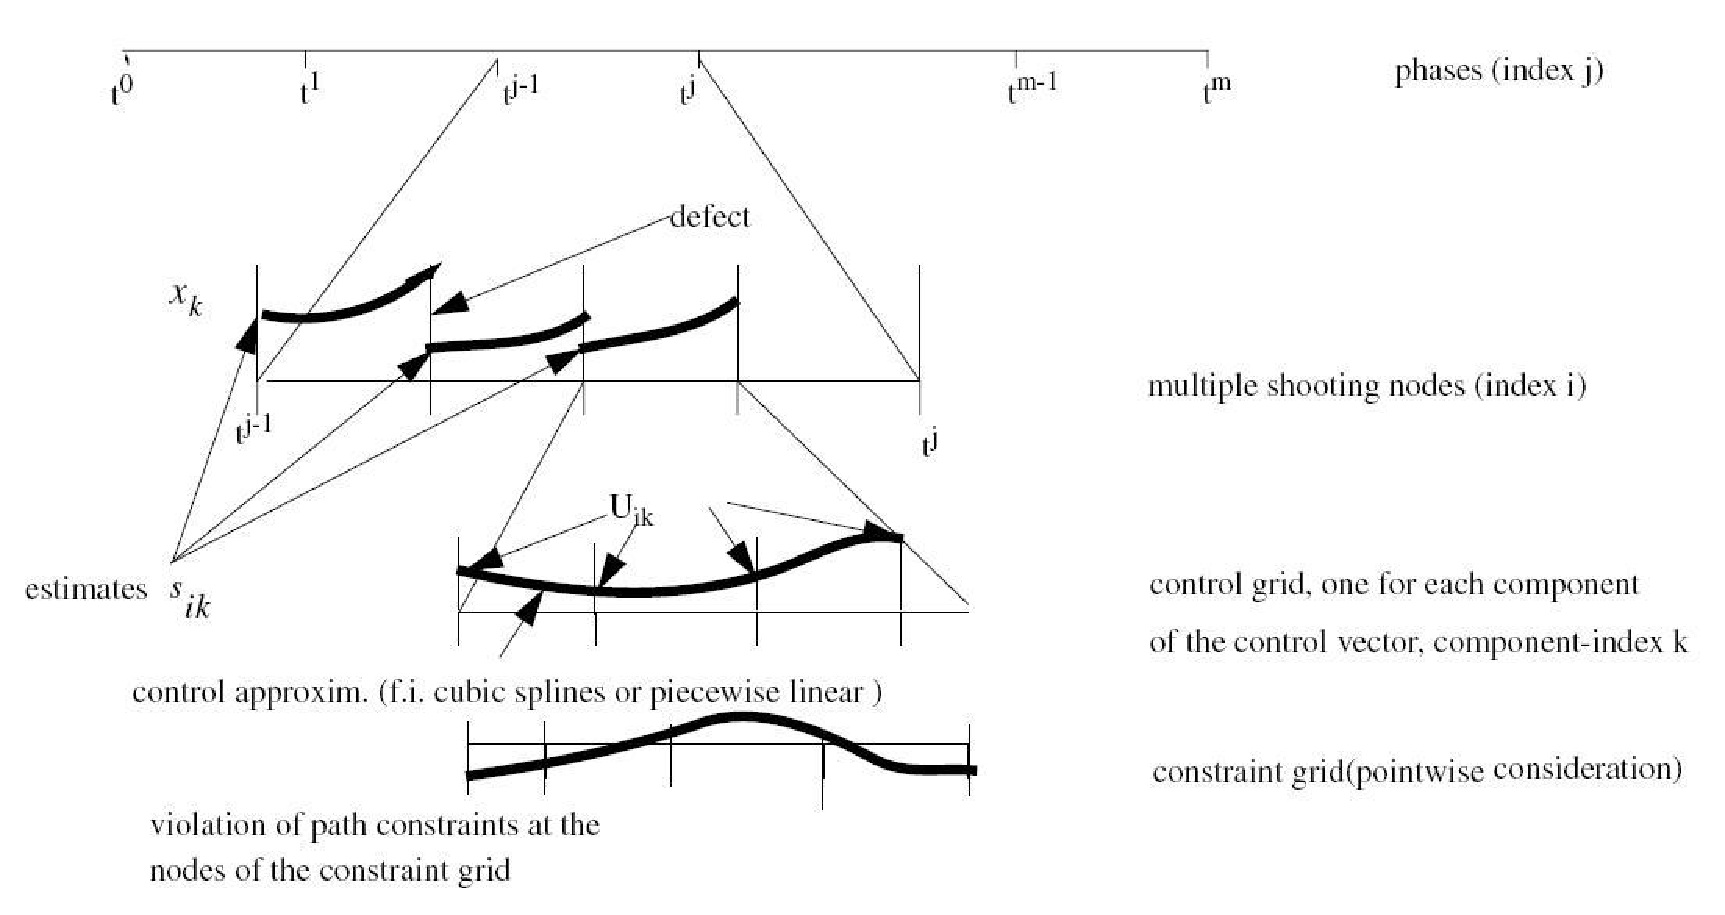
\includegraphics[width=\textwidth]{Images/control_nodes.pdf}
\end{center}
\caption{Optimisation grids. Image used courtesy of \textcite{ASTOS_guide}.}
\label{fig:Optimisation-grids}
\end{figure}

Between multiple shooting nodes a control grid allows addition of control discretisation points. Collocation requires that the multiple shooting nodes and control points match. Preliminary calculations for the \BW\ have been simulated with 80 major grid points in each phase (a second phase was added when the spacecraft is close to Earth-Moon Lagrange point 1 for better plotting). Since collocation methods have been used for \BW\ so far, no additional control points were added. Adding initial guesses for each of the optimisable parameters and states at each of the 80 major grid points results in about 40,000 parameters so far.

%Simulation
\subsection{Simulation} \label{sub:ASTOS-Simulation}

Following the initialisation, the mission scenario is then simulated based on the design parameters and initial guesses for all optimisable parameters. The integration method, integration error tolerances and number of output points are user-defined. For \BW\ a Runge-Kutta 4/5 method has been used as the most generic, robust variable-step integrator, with an error tolerance set to $1.0\times10^{-8}$. For the plotted trajectory to appear smooth requires about 1000 output
 points.

After integration, the results can be reviewed to ensure the initial guess is realistic (and should lead to a feasible optimum during the optimisation). Constrained parameters may also be reviewed throughout the simulation, to highlight any points where the contraint is violated (by default, during optimisation constraints are only evaluated at nodes to reduce the number of calculations required). Additional constraint evaluations may then be forced, to encourage the optimiser to remove the violation.

No additional constraint evaluations have been added for the \BW\ trajectory yet, since the only path constraints added were to prevent the spacecraft leaving the Earth-Moon system, an event that will not occur if the optimisation is behaving as expected.

% Optimisation
\subsection{Optimisation} \label{sub:ASTOS-Optimisation}

\textcite{ASTOS_guide} presents the case for the selection of optimisation algorithms CGA, TROPIC, PROMIS, CAMTOS and SOCS in ASTOS/GESOP. A brief summary of each of these methods is presented below.

\begin{itemize}
\item CGA (Constrained Genetic Algorithm) is an early implementation of a genetic algorithm, currently limited to integer parameters. It gives a better global search than the other implemented methods (all gradient based methods) but is not very computationally efficient, and was empirically shown to be ineffective for more than about 20 parameters, compared to the 40,000 already required for the simplified \BW\ scenario.
\item TROPIC (Trajectory OPtimisation by dIrect Collocation) and PROMIS (Parameterised tRajectory Optimisation by direct MultIple Shooting) are transcription methods developed at DLR. This means they transcribe the optimal control problem into a general Non-Linear Program (NLP). CAMTOS (Collocation And Multiple shooting Trajectory Optimisation Software) was developed internally by ASTOS Solutions. All three methods use Sequential Quadratic Programming (SQP) to solve the NLP. SQP attempts to solve the NLP by formulating and solving a series of quadratic sub-problems.

Two SQP methods are available. SLLSQP is a fairly generic SQP solver, and computes local optima in order $n^{3}$ time, where $n$ is the number of optimisable parameters. Consequently it is useful for scenarios with up to about 100 parameters. SNOPT (Sparse Nonlinear OPTimiser) was developed at Stanford University and incorporates a few modifications that exploit sparsity within the Jacobian matrix (non-linear parameters that may be treated as linear within the constrained region) allowing it to compute local optima in order $n^{2}$ time. Consequently it is more widely useful for up to about 1000 parameters.

\item The most recent version of ASTOS includes support for SOCS (Sparse Optimal Control Software), a combined transcription and SQP algorithm developed by The Boeing Company. SOCS is a direct collocation method that further exploits sparsity, resulting in a computational time that increases with order $n$. SOCS has successfully solved problems with over 500,000 parameters. Due to the long duration of \BW\ and the multitudinous optimisable parameters, SOCS is the preferred algorithm.
\end{itemize}

% Verification
\subsection{Verification} \label{sub:ASTOS-Verification}

The mathematics behind ASTOS has been well established for many decades \parencite{Kaplan1976}. The implementation within ASTOS itself has been numerically verified by ESTEC, Dassault, ASTRIUM, CNES, EADS and JAXA, among other industrial partners. It is practically validated by ongoing use on real missions launched by ESA and DLR, including Ariane 5 and Vega rocket launches, the ExoMars and Beagle 2 missions, and X38 re-entry scenarios.
 
Final results for the \BW\ optimisation will be further verified by simulating the trajectory in both Matlab and STK. While these packages will not verify that the solution is optimal, they will confirm that the solution is feasible, and can be used to compare trajectories on a case-by-case basis. The trajectory will receive final, practical verification when satellite is launched.

\section{Summary} \label{sec:Optimisation-Summary}

A variety of optimisation methods have been investigated, and a robust COTS software package that encapsulates several methods has been chosen to reduce development time. Unfortunately this package is limited to gradient based methods for complex multi-parameter scenarios, so rigourous analysis of initial conditions and basins of convergence will be required to ensure a global optimum is found. At present the package requires many simplifications for long duration low-thrust trajectories. Close cooperation will be required with the proprietors of the software to model the complexities and non-linearities involved with the \BW\ spacecraft.
 
\clearpage